
%________________________________________________________________________________________________

\chapter{Introduction}
\label{chap:intro}

\begin{tcolorbox}[width=\textwidth,colback={LightSteelBlue1}]
This chapter introduces the central verification problem of this thesis: \emph{reachability for local-timed negotiations}. It highlights the unique challenges posed by combining local time with multiparty interaction and provides a roadmap of the thesis, including (un)decidability results.
\end{tcolorbox}    

\noindent This chapter is motivational and structural. It tells the reader why the thesis matters and what its main results are. Chapter~\ref{chap:preliminaries} then provides the formal machinery used throughout the rest of the dissertation.

Concurrent systems rarely consist of a single thread of control evolving against a single clock. They are built from interacting components that proceed partly independently, occasionally coordinate, and often have quantitative timing requirements that matter for correctness. This thesis studies such systems through the model of \emph{local-timed negotiations} (LTNs), which combine explicit multiparty interaction with local real-time behavior. The central verification problem considered throughout is \emph{reachability}: given an initial configuration and a target control point, does there exist an execution that reaches the target while respecting the timing constraints of the model?

The thesis asks a structural question about this verification problem: \emph{what happens when concurrency is governed by explicit multiparty interaction, but time is local rather than global?} The answer is not a simple transfer of known timed-automata results. Once time is allowed to evolve independently for different agents and synchronization is made selective rather than implicit, reachability becomes markedly more expressive. In full generality, that expressiveness leads to undecidability. At the same time, the thesis shows that this negative result is not the end of the story. By imposing natural semantic or structural restrictions, one can recover decidability and obtain a precise landscape of tractable fragments.

This introduction is organized around that landscape. Section~\ref{sec:intro-motivation} motivates the need for a model that treats both timing and multiparty interaction as first-class. Section~\ref{sec:intro-positioning} places LTNs relative to timed automata and negotiations, but only at a high level; the formal machinery is deferred to Chapter~\ref{chap:preliminaries}. Section~\ref{sec:intro-ltns} presents the central modeling ideas behind LTNs and explains why local time fundamentally changes the verification picture. Section~\ref{sec:intro-contrib} summarizes the main results of the thesis and the overall decidability map. Sections~\ref{sec:intro-organization} and~\ref{sec:intro-related} close the chapter with the organization of the thesis and a brief discussion of related work.

%________________________________________________________________________________________________

\section{Motivation}
\label{sec:intro-motivation}

\subsection{Concurrency, time, and coordinated interaction}

In the world we live in, concurrency is ubiquitous. Imagine that we are walking inside a forest. Different birds, animals and insects are talking around us. Suddenly we see a beautiful bird peeping from a branch of a sunlit mossy tree. Our brain here is processing multiple sensory information, motor control, and cognition concurrently. Images, sounds, movement, forming memories, making a decision whether to capture this moment in our camera or not--- all are processed concurrently by different parts of our brain. At the same time, our heart rate, breathing, and reflexes are being controlled by other parts. These processes evolve largely independently, yet remain sufficiently coordinated to produce coherent behaviour. Such parallel activity illustrates a fundamental property of natural systems: concurrency. 

Natural systems process many forms of information in parallel, and engineered systems increasingly do the same. A mobile robot combines sensing, localization, planning, and actuation while interacting continuously with its environment. A communication protocol manages multiple sessions, timers, retransmissions, and acknowledgements concurrently. A medical device monitors physiological signals while coordinating diagnosis and control. Even when such systems are designed modularly, their correctness is rarely determined by the behavior of one component in isolation. It depends on how several components evolve together.

This observation has two consequences for formal modeling. First, a useful model of such systems must capture \emph{independent evolution}: components often make progress without waiting for one another. Second, it must capture \emph{coordination}: components sometimes need to interact in a structured way, and the form of that interaction matters. In many settings, that coordination is not merely pairwise. Several components may have to participate simultaneously in a joint interaction, commit to a common outcome, and then continue according to that joint decision.

Time adds a second layer of difficulty. In many systems, correctness is not purely qualitative. It is not enough that an event eventually happens; it must happen within a deadline, after a minimum delay, or in a precise order relative to other time-constrained activities. A collision-avoidance controller must combine sensor readings fast enough for braking decisions to be effective. A pacemaker must coordinate sensing and stimulation within tight time windows. A distributed protocol may tolerate independent local progress for some time, but later require the participants to synchronize before continuing. In such settings, time is not an annotation on top of behavior; it is part of the behavioral specification itself.

These two features—concurrency and quantitative time—have long been studied in formal verification through a variety of complementary models. Some provide especially natural descriptions of interaction structure, while others offer a direct treatment of quantitative timing constraints. Local-timed negotiations are motivated by bringing these perspectives together in a setting that makes both interaction patterns and local timing constraints explicit. The present thesis is motivated by the need for a model in which \emph{interaction structure}, \emph{local progress}, and \emph{timing} can all be represented explicitly.

\subsection{Why explicit multiparty interaction matters}

An important aspect of concurrent systems is that coordination often takes place
through interactions involving several agents at once. Classical state-based models often reduce multiparty interactions to combinations of smaller steps: shared variables, binary communications, or transitions whose effects are spread across an underlying state space. Such encodings are powerful, but they can hide the real coordination structure of a system. In verification, that hidden structure matters. It affects how independence is recognized, how state-space reductions are justified, and how one reasons about causality.

Negotiation-based models address this issue by taking \emph{atomic multiparty interaction} as primitive. A negotiation node specifies which agents participate, which outcomes are possible, and how those outcomes determine the subsequent local readiness of the participants. This style of modeling has two advantages for the present thesis. First, it makes concurrency explicit: two interactions with disjoint participant sets are structurally independent. Second, it makes synchronization explicit: if several agents have to act together, that requirement is visible in the model rather than emerging indirectly from a lower-level encoding.

Once time enters the picture, this distinction becomes even more important. In globally timed models, two actions that are structurally independent may nevertheless become coupled through the ambient passage of time. In interaction-centric models, by contrast, one can ask more finely \emph{when} time should matter jointly and \emph{when} it should remain local. This is one of the guiding ideas behind LTNs.

\begin{tcolorbox}[width=\textwidth, colback={LightGrey1}, colframe=black, title={A natural local-time intuition: flowering and pollination}, colbacktitle=LightGrey3, coltitle=black]
A useful way to think about local time is through temporal mismatch in natural
systems. Climate change may shift the local flowering schedule of plants without
producing the same shift in the emergence schedule of their pollinators. The
resulting problem is not simply that ``something happens late''; different
participants evolve according to partly separate local temporal rhythms, and
successful coordination depends on whether those rhythms align when interaction
becomes possible.

This thesis returns to that idea through a stylized pollination example. In
Chapter~\ref{chap:preliminaries}, the example is presented formally as a
negotiation in order to illustrate branching, delayed consequences of choice,
and the possible growth of the marking graph. At the motivational level,
however, the point is simpler: local time matters even in naturally
interaction-driven systems, and mismatches of local timing can be just as
important as the interaction structure itself. That intuition carries directly
into LTNs, where timing constraints may be local to different agents but their
consequences become visible at interactions.
\end{tcolorbox}    

\subsection{Verification and the reachability problem}

The practical motivation for studying concurrent real-time systems is clear: timing or coordination failures in such systems can have serious consequences, from protocol violations and service outages to safety-critical malfunction. The theoretical motivation is equally compelling. These systems lie at the intersection of several classical themes in formal methods---infinite-state verification, concurrency, partial-order reasoning, and real-time analysis---and they raise natural questions about the boundary between expressive power and algorithmic tractability.

Among verification problems, the most basic and most revealing one is \emph{reachability}. Given an initial configuration and a target configuration, is there an execution that reaches the target? Reachability already subsumes several familiar questions:
\begin{itemize}
    \item \textbf{Safety}: can a bad state be reached?
    \item \textbf{Deadlock detection}: can the system reach a configuration from which no further progress is possible?
    \item \textbf{Goal attainment}: can a desired control point, outcome, or marking be reached?
\end{itemize}
For this reason, reachability serves as a canonical benchmark for the algorithmic behavior of a model. If reachability is already undecidable, richer verification tasks inherit that hardness. If reachability is decidable, the proof techniques often reveal which aspects of the model are fundamentally responsible for tractability.

For concurrent systems, reachability is hard even without time. The source of this hardness is the familiar \emph{state-space explosion}: independent actions can interleave in many ways, causing the number of reachable states to grow rapidly. Partial-order reduction techniques mitigate this problem by exploiting commutativity of independent actions, thereby avoiding redundant exploration of behavior that differs only by interleaving.

Timed systems complicate this picture. Clocks can create dependencies between actions that would otherwise be independent, and global-time semantics may force components to advance together even when there is no direct interaction between them. As a result, the availability of partial-order reasoning depends heavily on how time is modeled. One of the motivations of this thesis is precisely to study a framework where structural independence is explicit and where synchronization of time is a modeling choice rather than a built-in semantic assumption.

\subsection{Why local time changes the question}

A natural way to add time to a concurrent model is to assume a single global notion of time. This is the classical approach in timed automata and in networks of timed automata: all clocks advance uniformly, and the system evolves against a shared temporal background. This choice is elegant and powerful, and it has led to a mature verification theory. But it is not the only meaningful way to model time.

In many distributed or loosely coupled systems, what matters operationally is not a single global time, but the local progression of time for each participant. Components may measure elapsed time relative to their own actions, their own deadlines, or their own waiting periods. They may proceed independently for long stretches and synchronize only at designated coordination points. In such a setting, treating time as inherently global can obscure the very patterns of independence one hopes to analyze.

Local-timed negotiations adopt the opposite viewpoint. Each agent evolves according to its own local reference time. Timing constraints are expressed through local clocks, and some interactions may additionally require participating agents to synchronize their local reference times. The result is a model in which both structural interaction and temporal coordination are explicit. This makes it possible to ask a more refined verification question: \emph{how much timing freedom can a concurrent system retain before reachability becomes undecidable?} The remainder of the chapter positions this question relative to existing models and summarizes the answer developed in the thesis.

%________________________________________________________________________________________________

\section{From timed automata and negotiations to local-timed negotiations}
\label{sec:intro-positioning}

Local-timed negotiations are best understood as arising from two complementary traditions. From timed automata they inherit quantitative timing constraints, real-valued clocks, guards, and resets. From negotiations they inherit an interaction-centric view of concurrency in which atomic multiparty interactions are primitive. The central contribution of the model is not merely to combine these ingredients syntactically, but to combine them under a \emph{local-time semantics} that preserves independence wherever synchronization is not explicitly required.

\subsection{Timed automata and the global-time paradigm}

Timed automata, introduced by Alur and Dill~\cite{AlurDillTA}, are one of the foundational models for real-time verification. A timed automaton is a finite-state control graph equipped with real-valued clocks. Transitions can test clocks against constants, reset selected clocks to zero, and thus express timing constraints such as deadlines, waiting periods, and response windows. The reachability problem asks whether a target state can be reached from the initial state by alternating time delays and discrete transitions.

The decisive feature of timed automata for the present discussion is that \emph{all clocks evolve with the same global time}. If a delay of length $\delta$ is taken, every clock increases by $\delta$.  Although the underlying state space is infinite and uncountable, one can pass to a finite abstraction via \emph{regions}; in practice, more efficient symbolic representations based on \emph{zones} are then used to explore reachable valuations algorithmically~\cite{AlurDillTA,DillPhD}.

The model is particularly successful when a system really is governed by a common global time, or when such a global-time view is a faithful abstraction. But from the point of view of true concurrency, the semantics has a cost: independent components are still coupled by the ambient flow of time. In a network of timed automata, two local components may be structurally unrelated and still advance together because delay transitions are global. This does not make the model less useful, but it does mean that the semantics of time already imposes a form of synchronization before any explicit synchronization action occurs.

For this thesis, timed automata serve both as inspiration and as a contrast. They provide the clock-based language in which local timing constraints will be expressed. At the same time, their standard semantics highlights the modeling decision that LTNs reject: the assumption that temporal progress is global by default.

Figure~\ref{fig:ab} shows an example timed automaton \(\mathcal{A}_1\) with two clocks \(x\) and \(y\), initial state \(q_0\), accepting state \(q_2\), and alphabet \(\{a,b\}\).

\begin{figure}[t]
\centering
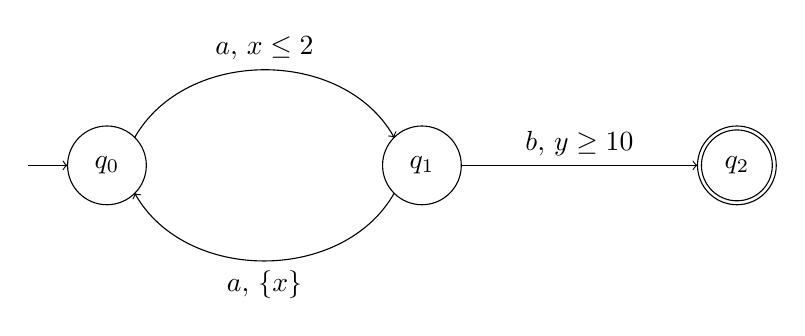
\begin{tikzpicture}[scale=1, every node/.style={transform shape}]

\filldraw [fill=white]  (0,0)  circle (5mm) node (q0) {$q_0$};
\filldraw [fill=white]  (4,0)  circle (5mm) node (q1) {$q_1$};
\filldraw [fill=white]  (8,0)  circle (5mm) node (q2) {$q_2$};
\draw (8,0)  circle (4.5mm);

\begin{scope}[->]
\draw (0.35,0.35) .. controls (1,1.5) and (3,1.5) .. (3.65,0.35) node [midway, above] {$a,\, x \leq 2$};
\draw (3.65,-0.35) .. controls (3,-1.5) and (1,-1.5) .. (0.35,-0.35) node [midway, below] {$a,\, \{x\}$};
\draw (4.5,0) -- (7.5,0) node [midway, above] {$b,\, y \geq 10$};
\draw (-1,0) -- (-0.5,0);
\end{scope}

\end{tikzpicture}
\caption{A timed automaton \(\mathcal{A}_1\). Both clocks \(x\) and \(y\) start at \(0\) in state \(q_0\). The transition on \(a\) from \(q_0\) to \(q_1\) has the guard \(x \leq 2\), forcing the system to spend at most \(2\) time units before taking it. The transition on \(a\) from \(q_1\) to \(q_0\) has no guard and resets \(x\). The guard on \(b\) from \(q_1\) to \(q_2\) requires that at least \(10\) time units have elapsed since the start, via the constraint \(y \geq 10\).}
\label{fig:ab}
\end{figure}
\begin{figure}[t]
\centering

\begin{tikzpicture}

\node at (0,0) {$(q_0, \langle 0, 0 \rangle)$};
\node at (-4,-2) {$(q_1, \langle 0, 0 \rangle)$};
\node at (0,-2) {$(q_1, \langle 0.8, 0.8 \rangle)$};
\node at (4,-2) {$(q_1, \langle 1.5, 1.5 \rangle)$};
\node at (-4,-4) {$(q_0, \langle 0, 0.8 \rangle)$};
\node at (0,-4) {$(q_0, \langle 0, 5.8 \rangle)$};
\node at (4,-4) {$(q_0, \langle 0, 9.8 \rangle)$};
\node at (0,-6) {$(q_1, \langle 0.5, 10.3 \rangle)$};
\node at (4,-6) {$(q_1, \langle 1.2, 11 \rangle)$};
\node at (8,-6) {$(q_1, \langle 1.8, 11.6  \rangle)$};
\node at (4,-8) {$(q_2, \langle 2.2, 12 \rangle)$};

\node at (-2,-2) {$\cdots$};
\node at (2,-2) {$\cdots$};
\node at (6,-2) {$\cdots$};
\node at (-2,-4) {$\cdots$};
\node at (2,-4) {$\cdots$};
\node at (6,-4) {$\cdots$};
\node at (-2,-6) {$\cdots$};
\node at (2,-6) {$\cdots$};
\node at (6,-6) {$\cdots$};
\node at (10,-6) {$\cdots$};
\node at (2,-8) {$\cdots$};
\node at (6,-8) {$\cdots$};
\node at (-4,-2.5) {$\vdots$};
\node at (4,-2.5) {$\vdots$};
\node at (-4,-4.5) {$\vdots$};
\node at (0,-4.5) {$\vdots$};
\node at (0,-6.5) {$\vdots$};
\node at (8,-6.5) {$\vdots$};

\begin{scope}[-Stealth]
\draw (0,-0.3) -- (-4,-1.7) node [midway, left, above] {\footnotesize $0$};
\draw (0,-0.3) -- (0,-1.7) node [midway, left] {\footnotesize $0.8$};
\draw (0,-0.3) -- (4,-1.7) node [midway, right, above] {\footnotesize $1.5$};
\draw (0,-2.3) -- (-4,-3.7) node [midway, left, above] {\footnotesize $0$};
\draw (0,-2.3) -- (0,-3.7) node [midway, left] {\footnotesize $5$};
\draw (0,-2.3) -- (4,-3.7) node [midway, right, above] {\footnotesize $9$};
\draw (4,-4.3) -- (0,-5.7) node [midway, left, above] {\footnotesize $0.5$};
\draw (4,-4.3) -- (4,-5.7) node [midway, left] {\footnotesize $1.2$};
\draw (4,-4.3) -- (8,-5.7) node [midway, right, above] {\footnotesize $1.8$};
\draw (4,-6.3) -- (4,-7.7) node [midway, left] {\footnotesize $1$};
\end{scope}

\end{tikzpicture}
\caption{Part of the transition system of the timed automaton \(\mathcal{A}_1\), showing several possible runs.}
\label{fig:ab-behavior}
\end{figure}

Figure~\ref{fig:ab-behavior} depicts part of the (infinite) transition system of \(\mathcal{A}_1\), showing some possible configurations and transitions. Starting from the initial configuration \((q_0, \langle 0,0 \rangle)\), the system may let time elapse in \(q_0\) for any duration between \(0\) and \(2\) units before taking the transition on \(a\) to \(q_1\). For instance, after \(0.8\) time units, the clock valuation becomes \(\langle 0.8, 0.8 \rangle\). Once in \(q_1\), the automaton can again delay, and may take the loop on \(a\) (resetting \(x\)) or eventually take the transition on \(b\) when \(y \ge 10\). Different choices of delay durations lead to uncountably many distinct runs.

\subsection{Negotiations and explicit multiparty synchronization}

Negotiations, introduced by Esparza and Desel~\cite{EsparzaDeselNegotiations}, provide a different starting point. They model concurrent behavior as a workflow of \emph{atomic negotiations}. Each negotiation node has a nonempty set of participating agents, called its domain, and a finite set of possible outcomes. When a node occurs, all agents in its domain participate jointly, agree on one of the available outcomes, and update their future readiness accordingly.

This style of modeling makes two aspects of concurrency transparent. First, it makes \emph{synchronization} explicit: if a node involves agents $p$, $q$, and $r$, then the interaction among them is atomic and visible at the top level of the model. Second, it makes \emph{independence} explicit: nodes with disjoint domains can proceed independently.

Operationally, the state of a negotiation is given by a \emph{marking}, which records, for each agent, the set of nodes that the agent is currently ready to participate in. A node is enabled if all its participating agents are ready for it. When an enabled node occurs with a chosen outcome, the readiness sets of the participating agents are updated according to the outcome, while the readiness of non-participants remains unchanged. The reachability problem then asks whether a target marking, outcome, or control point can be reached from the initial marking.

Negotiations provide a convenient starting point for the present thesis. They can be used to describe workflows, distributed protocols, and structured coordination patterns, and they are naturally related to workflow Petri nets and business-process models~\cite{EsparzaWorkflow,EsparzaFreeChoice}. For our purposes, the key point is that they represent \emph{multiparty} interaction directly. This gives a clear structural layer to which local quantitative timing constraints can later be added.

\subsection{A running example: an ATM workflow}

To illustrate the graphical notation for negotiations, Figure~\ref{fig:node}
shows a single node \(n\) with domain \(\{p_1,p_2,p_3\}\) and one outcome \(r\).
The thick horizontal bar represents the atomic interaction, the white circles
indicate the participating processes, and the outgoing arcs labelled \(r\)
describe how readiness is updated after that outcome occurs.

%To illustrate the negotiation viewpoint, consider a simple ATM scenario with three agents: a customer $c$, the ATM machine $a$, and the bank $b$. The interaction proceeds through several atomic negotiations. First, all three agree to start the transaction. Then the customer and the ATM interact to submit the request. After that, the ATM and the bank interact to forward the relevant details. Finally, all three synchronize again to decide whether the request succeeds or fails.

%This small example already exhibits the key structural features of negotiations. Some interactions are \emph{pairwise}, involving only two of the agents at a time. Others are \emph{joint} and require a multiparty synchronization. The control flow of the system is determined not by a monolithic global state but by the distribution of local readiness among the agents.

\begin{figure}[t]
\centering
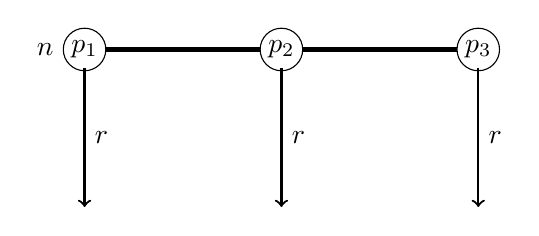
\begin{tikzpicture}

\begin{scope}[line width=2pt]
\draw (0,0) node at (-0.5,0) {$n$} -- (5,0);
\end{scope}

\begin{scope}[fill=white]
\filldraw  (0,0)  circle (2.7mm) node (nic) {$p_1$};
\filldraw  (2.5,0)  circle (2.7mm) node (nia) {$p_2$};
\filldraw  (5,0)  circle (2.7mm) node (nib) {$p_3$};
\end{scope}

\begin{scope}[thick,->]

\draw (nic) -- (0,-2) node [right, midway] {$r$};
\draw (nia) -- (2.5,-2) node [right, midway] {$r$};
\draw (nib) -- (5,-2) node [right, midway] {$r$};
\end{scope}

\end{tikzpicture}
\caption{A simple node $n$ with three processes $\{p_1, p_2, p_3\}$ in its domain, and the set of outcomes is $\{r\}$}
\label{fig:node}
\end{figure}

\subsubsection{A simple example: ATM workflow}
\label{example:ATM-untimed}

Before presenting a more elaborate scenario, we introduce negotiations through a simple example. Consider a transaction in an ATM machine ($a$), where a customer ($c$) wants to withdraw money from her bank ($b$).  Here, $a$, $c$, and $b$ are the \emph{processes} in the system. Their direct interactions are represented by thick horizontal lines (nodes). After each interaction, the participating agents decide on an outcome, represented by arrows. Initially, all agents are in the node $n_{in}$ node. They choose the outcome $st$ to start the transaction. Agents $a$ and $c$ go to node $n_1$ and $b$ goes to $n_2$.The customer gives her card details and requests for money withdrawal in the ATM at node $n_1$ by the outcome $req$. At $n_2$, the ATM conveys this request to the bank and sends the details through the outcome $det$. All three processes talk to each other at $n_3$, where the bank checks if there is sufficient money in the account and let the customer know via the ATM. They select $ok$ if the transaction is approved and go to $n_f$ otherwise they go back to $n_{in}$ by choosing the outcome $fail$.

\begin{figure}[t]
\centering
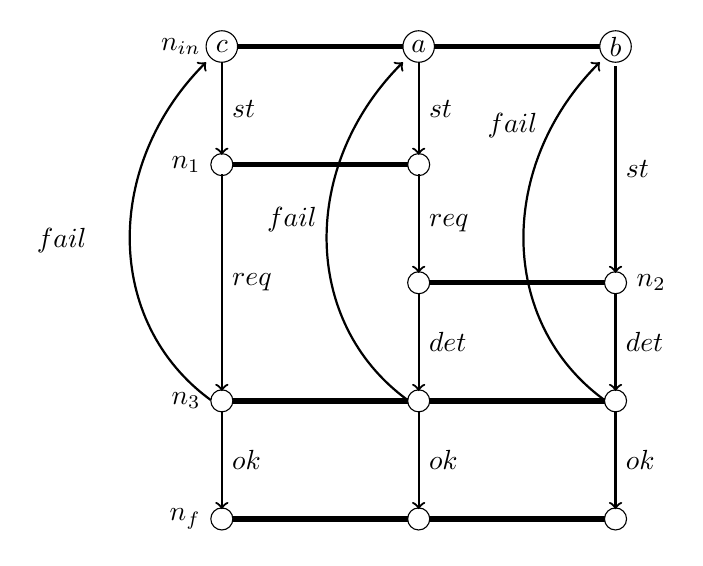
\begin{tikzpicture}

\begin{scope}[line width=2pt]
\draw (0.,0) node [left] {$n_{in}\,\,$} -- (5,0);
\draw (0.,-1.5) node [left] {$n_{1}\,\,$} -- (2.5,-1.5);
\draw (2.5,-3) -- (5,-3) node [right] {$\,\,n_{2}$};
\draw (0.,-4.5) node [left] {$n_{3}\,\,$} -- (5,-4.5);
\draw (0.,-6) node [left] {$n_{f}\,\,$} -- (5,-6);
\end{scope}

\begin{scope}[fill=white]
\filldraw  (0,0)  circle (2mm) node (nic) {$c$};
\filldraw  (2.5,0)  circle (2mm) node (nia) {$a$};
\filldraw  (5,0)  circle (2mm) node (nib) {$b$};

\filldraw  (0,-1.5)  circle (1.4mm) node (n1c) {};
\filldraw  (2.5,-1.5)  circle (1.4mm) node (n1a) {};

\filldraw  (2.5,-3)  circle (1.4mm) node (n2a) {};
\filldraw  (5,-3)  circle (1.4mm) node (n2b) {};

\filldraw  (0,-4.5)  circle (1.4mm) node (n3c) {};
\filldraw  (2.5,-4.5)  circle (1.4mm) node (n3a) {};
\filldraw  (5,-4.5)  circle (1.4mm) node (n3b) {};

\filldraw  (0,-6)  circle (1.4mm) node (n4c) {};
\filldraw  (2.5,-6)  circle (1.4mm) node (n4a) {};
\filldraw  (5,-6)  circle (1.4mm) node (n4b) {};
\end{scope}

\begin{scope}[thick,->]

\draw (nic) -- (n1c) node [right, midway] {$st$};
\draw (n1c) -- (n3c) node [right, midway] {$req$};
\draw (n3c) -- (n4c) node [right, midway] {$ok$};

\draw (nia) -- (n1a) node [right, midway] {$st$};
\draw (n1a) -- (n2a) node [right, midway] {$req$};
\draw (n2a) -- (n3a) node [right, midway] {$det$};
\draw (n3a) -- (n4a) node [right, midway] {$ok$};

\draw (nib) -- (n2b) node [right, midway] {$st$};
\draw (n2b) -- (n3b) node [right, midway] {$det$};
\draw (n3b) -- (n4b) node [right, midway] {$ok$};

\draw (n3c) + (-0.14,0.01) .. controls  (-1.5,-3.5) and (-1.5,-1.5) .. (nic) node [left=-0.2cm, text width = 1.25 cm, midway] {$fail$};
\draw (n3a) + (-0.14,0.01) .. controls  (1,-3.5) and (1,-1.5) .. (nia) node at (1.2,-2.2) [text width = 1.25 cm] {$fail$};
\draw (n3b) + (-0.14,0.01) .. controls  (3.5,-3.5) and (3.5,-1.5) .. (nib) node at (4,-1) [text width = 1.25 cm] {$fail$};

\end{scope}

\end{tikzpicture}
\caption{A distributed negotiations modelling a transaction between a customer, an ATM and a bank}
\label{fig:ATM}
\end{figure}

This example is also useful conceptually because it foreshadows the timed extension. In an untimed negotiation, the ATM scenario captures \emph{who} interacts with whom and \emph{in what order} outcomes are possible. What it does not capture is that the customer may wait only so long before giving up, or that the bank may require an OTP to be validated within a limited time window. Introducing such constraints while keeping time local to the relevant participants is precisely the role of LTNs.

\subsection{Why combining the two models is not routine}

At first sight, one might expect that adding clocks to negotiations is straightforward: attach guards and resets to outcomes, let clocks evolve, and inherit the verification theory from timed automata. The thesis shows that this expectation is false. The key reason is semantic.

If one were to add clocks to negotiations while keeping a global-time semantics, the resulting model would collapse toward a timed-automata-like product construction. All agents would still advance under the same delay, and multiparty interaction would be timed against a shared global clock. This produces a meaningful model, but not the one studied here.

LTNs instead assign a local reference time to each agent and allow those reference times to evolve independently. Some interactions may then require the participating agents to synchronize their reference times, while others do not. Once this selective synchronization is permitted, a new phenomenon appears: relative timing differences between agents can accumulate, persist, and later be compared or eliminated through synchronizing interactions. This is exactly the phenomenon that drives the negative results of the thesis.

Thus LTNs are not simply ``timed negotiations.'' They are negotiations enriched with a \emph{local-time semantics} under which synchronization itself becomes part of the expressive power of the model.

\subsection{A compact comparison of the three viewpoints}

The contrast among timed automata, negotiations, and LTNs can be summarized informally as follows.

\begin{center}
\begin{tabular}{p{3.1cm}p{3.6cm}p{3.8cm}p{3.8cm}}
\toprule
\textbf{Model} & \textbf{What is primitive?} & \textbf{How does time evolve?} & \textbf{What is explicit?} \\
\midrule
Timed automata & local control transitions with guards and resets & globally, through a shared delay semantics & timing constraints; less explicit concurrency structure \\
Negotiations & atomic multiparty interaction and outcomes & not modeled quantitatively & synchronization and independence in the control structure \\
Local-timed negotiations & atomic multiparty interaction plus local timing constraints & locally, per agent; synchronization optional at selected nodes & both interaction structure and temporal coordination \\
\bottomrule
\end{tabular}
\end{center}

This table captures the conceptual niche of LTNs. They are designed to expose exactly the interaction between explicit concurrency and local time that is hidden in one direction by untimed negotiation models and in the other by global-time real-time models.

%________________________________________________________________________________________________

\section{Local-timed negotiations at a glance}
\label{sec:intro-ltns}

This section presents the central ideas of LTNs informally. The full syntax and semantics are given in Chapter~\ref{chap:ltn}; here the goal is to give a clear conceptual picture of what the model adds and why the reachability problem becomes interesting.

\subsection{Local reference time and local clocks}

Each agent in an LTN has its own \emph{local reference time}. Intuitively, this is the agent's own notion of elapsed time as the system executes. In addition, each agent may carry ordinary local clocks, which evolve with that agent's reference time and can be tested or reset at negotiation outcomes. In this way, LTNs preserve the familiar clock-based language of timed automata while changing the ambient temporal semantics.

Two kinds of timing information are therefore present:
\begin{itemize}
    \item \textbf{Local clocks}, which are used in guards and can be reset, and
    \item \textbf{Reference times}, which record the agent's accumulated local time and are used to define synchronization.
\end{itemize}

The essential design choice is that reference times are not assumed to evolve in lockstep. Between interactions, one agent may accumulate more local time than another. This means that the system retains genuine temporal asynchrony even while maintaining a structured interaction graph.

\subsection{Time-synchronizing and non-synchronizing interactions}

A negotiation node in an LTN still represents an atomic multiparty interaction, but it may now come in one of two flavors.

A \emph{non-synchronizing} interaction behaves like an ordinary timed local step embedded in a negotiation node: the participating agents must satisfy the relevant local clock guards, and the outcome may reset some clocks, but their reference times need not be equal. The interaction respects their local temporal histories without forcing alignment.

A \emph{time-synchronizing} interaction adds an equality constraint on the participating agents' reference times. Such an interaction can occur only when the participants have aligned their local times, and once it occurs, the alignment becomes an explicit part of the execution. This is the mechanism that allows LTNs to model both loosely coupled and tightly coordinated behavior inside the same framework.

Seen this way, LTNs do not simply attach clocks to a concurrent model. They distinguish between two notions that are conflated in standard global-time semantics:
\begin{enumerate}
    \item \emph{time passing}, and
    \item \emph{agents being temporally aligned}.
\end{enumerate}
In LTNs, time may pass without alignment, and alignment may be required only at chosen interactions.

\subsection{A timed reading of the ATM example}

Return to the ATM scenario. Suppose that after the customer initiates the transaction, the ATM must receive the customer's response within a bounded local time window, while the bank requires that an OTP validation complete within another local deadline. Under a global-time semantics, such requirements would be phrased against a single shared time axis. Under LTNs, they can instead be expressed against the local clocks of the relevant agents.

For instance, the customer may carry a clock that is reset when the request is issued and later checked when the OTP is entered. The bank may carry a different clock, reset when the OTP is sent and checked when validation occurs. These constraints are local: they refer to the temporal obligations of the relevant agents. If a later interaction additionally requires the ATM and the bank to be temporally aligned, that is modeled through a time-synchronizing negotiation node. Thus the model distinguishes between \emph{having a local deadline} and \emph{having to synchronize local time with another participant}.

This distinction is the source of both the expressive strength and the verification complexity of LTNs.

\begin{figure}[t]
  \centering
  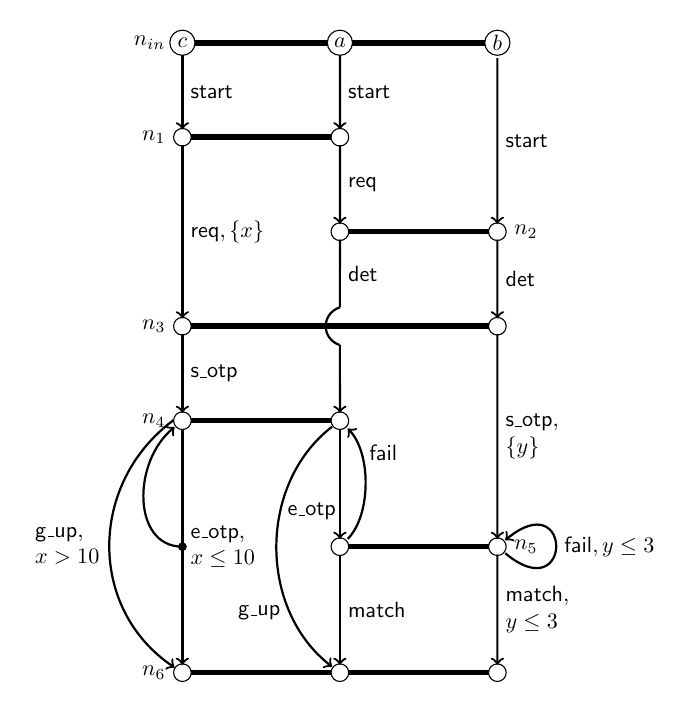
\begin{tikzpicture}[scale=0.8, every node/.style={transform shape}]

\begin{scope}[line width=2pt]
  \draw (0.,0) node [left] {$n_{\text{in}}\,\,$} -- (5,0); 
  \draw (0.,-1.5) node [left] {$n_{1}\,\,$} -- (2.5,-1.5); 
  \draw (2.5,-3) -- (5,-3) node [right] {$\,\,n_{2}$}; 
  \draw (0.,-4.5) node [left] {$n_{3}\,\,$} -- (5,-4.5); 
  \draw (0.,-6) node [left] {$n_{4}\,\,$} -- (2.5,-6); 
  \draw (2.5,-8) -- (5,-8) node [right] {\,\,$n_{5}$}; 
  \draw (0.,-10) node [left] {$n_{6}\,\,$} -- (5,-10);
\end{scope}

\begin{scope}[fill=white]
  \filldraw (0,0) circle (2mm) node (nic) {$c$}; 
  \filldraw (2.5,0) circle (2mm) node (nia) {$a$}; 
  \filldraw (5,0) circle (2mm) node (nib) {$b$};

  \filldraw (0,-1.5) circle (1.4mm) node (n1c) {}; 
  \filldraw (2.5,-1.5) circle (1.4mm) node (n1a) {};

  \filldraw (2.5,-3) circle (1.4mm) node (n2a) {}; 
  \filldraw (5,-3) circle (1.4mm) node (n2b) {};

  \filldraw (0,-4.5) circle (1.4mm) node (n3c) {}; 
  \filldraw (5,-4.5) circle (1.4mm) node (n3b) {};

  \filldraw (0,-6) circle (1.4mm) node (n4c) {}; 
  \filldraw (2.5,-6) circle (1.4mm) node (n4a) {};

  \filldraw (2.5,-8) circle (1.4mm) node (n5a) {}; 
  \filldraw (5,-8) circle (1.4mm) node (n5b) {};

  \filldraw (0,-10) circle (1.4mm) node (n6c) {}; 
  \filldraw (2.5,-10) circle (1.4mm) node (n6a) {}; 
  \filldraw (5,-10) circle (1.4mm) node (n6b) {};

  \filldraw [fill=black] (0,-8) circle (0.6mm) node (v1) {};
\end{scope}

\begin{scope}[thick,->]
  \draw (nic) -- (n1c) node [right, midway] {$\mathsf{start}$}; 
  \draw (n1c) -- (n3c) node [right, midway] {$\mathsf{req}, \{x\}$}; 
  \draw (n3c) -- (n4c) node [right, midway] {$\mathsf{s\_otp}$}; 
  \draw (n4c) -- (n6c) node [right, text width = 1.2 cm, midway] {$\mathsf{e\_otp},$ $x\leq10$}; 
  \draw (0,-8) .. controls (-0.8,-8) and (-0.8,-6.65) .. (n4c);

  \draw (nia) -- (n1a) node [right, midway] {$\mathsf{start}$}; 
  \draw (n1a) -- (n2a) node [right, midway] {$\mathsf{req}$}; 
  \draw (2.5,-4.8) -- (n4a); 
  \draw (n4a) -- (n5a) node [left=-0.3cm, text width = 1 cm, near end] {$\mathsf{e\_otp}$}; 
  \draw (n5a) -- (n6a) node [right, text width = 1 cm, midway] {$\mathsf{match}$}; 
  \draw (n5a) .. controls (3,-7.5) and (3,-6.5) .. (n4a) node [right, near end] {$\mathsf{fail}$}; 
  \draw (n4a) .. controls (1.2,-7) and (1.2,-9) .. (n6a) node [left=-0.3cm, text width = 1 cm, near end] {$\mathsf{g\_up}$};

  \draw (nib) -- (n2b) node [right, midway] {$\mathsf{start}$}; 
  \draw (n2b) -- (n3b) node [right, midway] {$\mathsf{det}$}; 
  \draw (n3b) -- (n5b) node [right, text width = 1 cm, midway] {$\mathsf{s\_otp},$ $\{y\}$}; 
  \draw (n5b) -- (n6b) node [right, text width = 1 cm, midway] {$\mathsf{match},$ $y\leq3$}; 
  \draw (n5b) .. controls (6.2,-9) and (6.2,-7) .. (n5b) node [right, midway] {$\mathsf{fail}, y\leq3$};

  \draw (n4c) + (-0.14,0.01) .. controls (-1.5,-7) and (-1.5,-9) .. (n6c) node [left=-0.2cm, text width = 1.25 cm, midway] {$\mathsf{g\_up},$ $x > 10$};
\end{scope}

\draw [thick] (n2a) -- (2.5,-4.2) node [right, midway] {$\mathsf{det}$}; 
\draw [thick] (2.5,-4.2) .. controls (2.2,-4.3) and (2.2,-4.7) .. (2.5,-4.8);
\end{tikzpicture}
\caption{ATM transaction as a local-timed negotiation. Customer $c$ has local clock $x$ (reset at $\mathsf{req}$, checked at $\mathsf{e\_otp}$ and $\mathsf{g\_up}$). Bank $b$ has local clock $y$ (reset at $\mathsf{s\_otp}$, checked at $\mathsf{match}$ and $\mathsf{fail}$). Annotations like "$x \leq 10$" are guards; "$\{x\}$" indicates clock reset.}
\label{fig:ATM}
\end{figure}

\subsection{Why local time is attractive}

The local-time semantics of LTNs is not only mathematically interesting; it is also conceptually attractive for several modeling reasons.

\paragraph{Explicit independence.}
If two negotiation nodes involve disjoint sets of agents and neither node synchronizes time, then their temporal progress is genuinely independent. There is no hidden global-time coupling forcing them to advance in lockstep.

\paragraph{Closer to distributed intuition.}
In distributed systems, different components often measure time locally. Even when a physical global time exists, algorithms are typically written against local timers, local waiting periods, and local deadlines. LTNs reflect this modeling stance directly.

\paragraph{Selective coordination.}
Real systems rarely sit at one of two extremes---fully asynchronous or fully synchronous. They are often partly one and partly the other. LTNs support this by allowing time-synchronization to be attached only to selected interactions.

\paragraph{Potential for partial-order reasoning.}
Because the model preserves structural independence rather than erasing it under a global-time semantics, it invites connections with partial-order methods. Although such algorithmic developments lie mostly beyond the scope of this thesis, the model is designed in a way that keeps this avenue open.

\subsection{Why local time is difficult}

The same feature that makes LTNs expressive also makes verification difficult. Once local reference times can diverge and later be required to align, the system can use relative timing differences as a form of stored information. Informally:
\begin{itemize}
    \item a non-synchronizing phase allows agents to drift apart in local time,
    \item a later time-synchronizing interaction can compare or constrain that drift,
    \item and the alternation of these two behaviors can simulate unbounded computation.
\end{itemize}

This is the conceptual core of the undecidability result proved later in the thesis. It also explains the structure of the positive results: each decidable fragment works by disabling, bounding, or structurally controlling this interplay between \emph{drift} and \emph{synchronization}.

The contribution of the thesis is therefore not merely to define LTNs, but to identify the precise conditions under which their reachability problem becomes tractable.

%________________________________________________________________________________________________

\section{Contributions and main results}
\label{sec:intro-contrib}

This thesis provides a systematic study of the decidability and complexity of reachability for local-timed negotiations. Its main results can be read as a map of what happens when one varies the strength of synchronization and the extent to which local times can diverge.

\subsection{The central negative result}

The first main result is that general LTNs are too expressive for decidable reachability. When time-synchronizing and non-synchronizing interactions can be mixed arbitrarily, the model can encode unbounded computation. The proof, developed in Chapter~\ref{chap:ltn}, gives a reduction from two-counter machines. At a high level, counter values are represented by differences between local reference times, while selective synchronization is used to compare or transfer these differences.

This shows that the difficulty of LTNs is not due merely to the presence of clocks. Rather, it is the combination of three features that matters:
\begin{enumerate}
    \item local evolution of time,
    \item persistence of relative timing differences, and
    \item selective synchronization that can later constrain those differences.
\end{enumerate}

This result provides the negative boundary against which all later decidability results are measured.

\subsection{Decidable extremes of the synchronization spectrum}

The thesis then identifies two structurally extreme fragments in which reachability becomes decidable and, in fact, PSPACE-complete.

\paragraph{Synchronization-free LTNs.}
In this fragment, no interaction synchronizes local reference times. Agents still carry local clocks and can still be constrained by local guards, but there is no mechanism for comparing their accumulated temporal drift. The reachability analysis can therefore be organized via a product-style region abstraction across agents, leading to PSPACE-completeness.

\paragraph{Always-synchronizing LTNs.}
At the opposite extreme, every interaction synchronizes local reference times. In this setting, the local-time semantics collapses toward a global-time behavior: although the model remains interaction-centric, every reachable target admits a monotone witness run that can be interpreted through a timed-automata-style analysis. Reachability is again PSPACE-complete.

These two results are important conceptually. They show that undecidability does not come from local time alone, nor from synchronization alone. It arises from the \emph{combination} of independent drift and selective synchronization.

\subsection{Decidability via bounded drift}

Between the two synchronization extremes lies a broader semantic class: \emph{drift-bounded LTNs}. Informally, an LTN is drift-bounded if every discrete behavior admits some timed realization in which the difference between local reference times never grows beyond a fixed constant.

This is a natural intermediate notion. It allows selective synchronization and local-time evolution to coexist, but forbids them from generating unbounded temporal divergence. The thesis shows that this condition is sufficient to recover a finite abstraction and hence decidability of reachability. For fixed drift bound $k$, the resulting problem is PSPACE-complete. Chapter~\ref{chap:drift-bounded} also studies the meta-problem of deciding drift boundedness itself and analyzes the special case of acyclic LTNs, where acyclicity implies bounded drift and yields an NP-complete reachability problem.

Thus drift-boundedness plays two roles in the thesis: it provides both a semantic explanation of why some fragments are decidable and a bridge between the undecidable general model and the structurally restricted classes that follow.

\subsection{Decidability via communication structure}

The final major contribution is a structural fragment called \emph{connectedly-communicating LTNs}. Here the restriction is not stated directly in terms of time, but in terms of how synchronization is distributed across loops in the marking graph. Roughly speaking, every cyclic behavior must contain enough synchronizing communication to connect the participating agents.

The intuition is that if all agents in a loop are repeatedly tied together through synchronization paths, then no one agent can drift arbitrarily far away without that drift eventually being absorbed by the rest of the system. The thesis formalizes this idea through communication graphs on loops and proves that connectedly-communicating LTNs are drift-bounded. Decidability of reachability then follows from the drift-bounded framework.

This result is particularly important because it shows that decidability can be recovered not only by bounding time semantically, but also by imposing a natural structural condition on how synchronization is arranged in the control graph.

\subsection{A summary of the landscape}

Taken together, the main results of the thesis can be summarized as follows.

\begin{center}
\begin{tabular}{p{5.0cm}p{3.2cm}p{4.0cm}}
\toprule
\textbf{Fragment} & \textbf{Reachability} & \textbf{Main reason} \\
\midrule
General LTNs with mixed synchronization & Undecidable & unbounded drift can be created and later tested \\
Synchronization-free LTNs & PSPACE-complete & drift exists but cannot be compared via synchronization \\
Always-synchronizing LTNs & PSPACE-complete & drift cannot persist across interactions \\
$k$-drift-bounded LTNs & PSPACE-complete (fixed $k$) & relative timing differences stay finitely representable \\
Acyclic LTNs & NP-complete & acyclicity prevents unbounded accumulation of drift \\
Connectedly-communicating LTNs & Decidable & communication structure forces bounded drift \\
\bottomrule
\end{tabular}
\end{center}

This table is more than a list of results. It expresses the central explanatory thesis of the dissertation: \emph{reachability in LTNs becomes hard precisely when relative timing information can accumulate without bound and later be interrogated by selective synchronization}. Each decidable fragment removes or controls one side of that mechanism.

\subsection{What is conceptually new in the thesis}

Beyond the individual complexity results, the thesis contributes a perspective on timed concurrency built around three axes:
\begin{enumerate}
    \item whether time is global or local,
    \item whether synchronization is absent, selective, or pervasive, and
    \item whether relative timing information can persist across interactions.
\end{enumerate}
LTNs inhabit the part of this design space where time is local, synchronization is explicit, and relative timing differences may persist. The results of the thesis then show how restrictions along these axes delineate the boundary between decidability and undecidability.

This perspective is one of the main conceptual contributions of the work. It makes clear that the interesting verification question is not simply ``what is the complexity of a new timed model?'' but rather ``which combinations of concurrency structure and temporal coordination preserve algorithmic tractability?''

%________________________________________________________________________________________________

\section{Organization of the thesis}
\label{sec:intro-organization}

The thesis is divided into two parts.

\paragraph{Part~I: introducing the model and establishing the negative boundary.}
Chapter~\ref{chap:preliminaries} collects the technical background needed later. It recalls negotiations, timed automata, and networks of timed automata, together with the notation and semantic conventions used throughout the dissertation. The chapter is intentionally foundational: it provides the formal toolkit against which LTNs are introduced.

Chapter~\ref{chap:ltn} then defines local-timed negotiations formally. It presents the local-time semantics, explains the role of local clocks and time-synchronizing nodes, and studies the expressive phenomena that arise from this semantics. The main technical result of the chapter is the undecidability of reachability for general LTNs.

\paragraph{Part~II: decidable subclasses.}
Chapter~\ref{chap:synch-fragments} begins the positive side of the story by studying the two synchronization extremes. It shows that both synchronization-free LTNs and always-synchronizing LTNs have PSPACE-complete reachability, but for fundamentally different reasons.

Chapter~\ref{chap:drift-bounded} moves beyond these extremes by introducing drift-bounded LTNs. It develops the region-style abstraction used for bounded drift, proves decidability and complexity results for that fragment, and analyzes acyclic LTNs as a structurally simpler special case.

Chapter~\ref{chap:connected-communicating} studies connectedly-communicating LTNs. It introduces communication graphs on loops in the marking graph, develops the tightening and propagation arguments needed to control temporal divergence, and proves decidability of reachability for this structurally defined fragment.

\paragraph{Conclusion and outlook.}
Chapter~7 summarizes the overall picture that emerges from the thesis and discusses broader directions, including quantitative extensions, structural parameters, and possible connections to other infinite-state models.

\paragraph{How to read the thesis.}
A reader primarily interested in the main results can read this introduction, then Chapter~\ref{chap:ltn} for the model and the undecidability result, and finally Chapters~\ref{chap:synch-fragments}--\ref{chap:connected-communicating} for the decidable fragments. A reader interested in the technical foundations behind the constructions and comparisons should read Chapter~\ref{chap:preliminaries} first.

%________________________________________________________________________________________________

\section{Related work}
\label{sec:intro-related}

The thesis sits at the intersection of several research strands: local-time semantics for real-time systems, timed models of concurrency, negotiation-based models, and structurally restricted distributed systems. This section briefly positions LTNs relative to those lines of work.

\subsection{Timed automata and local-time semantics}

Timed automata~\cite{AlurDillTA} and their symbolic verification theory form one of the main foundations of the present work. The use of clocks, guards, resets, and region-style reasoning in LTNs is directly inspired by this tradition. Symbolic representations based on zones and difference-bound matrices~\cite{DillPhD} have also strongly influenced how real-time reachability is usually approached, even though the present thesis is more concerned with decidability and complexity than with implementation.

A more specific point of contact is the \emph{local-time semantics} for networks of timed automata~\cite{LocalTimeTA}. In that setting, local progress and partial-order structure become more visible than under the standard global-time semantics. Subsequent work has used this viewpoint for zone-based reachability~\cite{LocalZone1,LocalZone2} and for B\"uchi-style analyses~\cite{LocalBuchi}. LTNs differ from these approaches in an important way: the local-time viewpoint is not an alternative semantics layered on top of another model, but is built into the very definition of the system. Moreover, synchronization in LTNs is explicit at the level of negotiation nodes, rather than emerging solely from shared actions.

\subsection{Timed concurrency models beyond timed automata}

A broad range of formalisms combine concurrency and quantitative time, including time Petri nets~\cite{MerlinTimePN}, timed-arc Petri nets~\cite{HansenTimedArc}, and time-constrained message sequence charts~\cite{AlurMSC}. These models vary in how they represent synchronization, causality, and the passage of time. Some support strong structural reasoning; others favor symbolic timing analysis. LTNs belong to this general family of timed-concurrency models, but differ in taking \emph{multiparty interaction} as primitive and in separating local temporal evolution from synchronization.

Partial-order methods for timed systems have also been studied extensively, for instance through unfoldings and related abstractions~\cite{EsparzaUnfoldings,KhomenkoTimePN}. These works share a guiding concern with the present thesis: to retain as much independence structure as possible while still reasoning effectively about time. LTNs contribute to this agenda from the angle of interaction-centric modeling.

\subsection{Negotiations and workflow-style concurrency}

Negotiations themselves were introduced as a concurrency model centered on atomic multiparty interactions~\cite{EsparzaDeselNegotiations}. Their theory has been developed in connection with soundness, summarization, and the analysis of workflow-style behavior, and they have close links to workflow Petri nets and business-process models~\cite{EsparzaWorkflow,EsparzaFreeChoice}. This connection is part of what makes negotiations a natural base model for timed extensions: they already support structured distributed coordination with explicit synchronization and visible independence.

To the best of our knowledge, local-timed negotiations as studied in this thesis were first proposed in~\cite{LTNOriginal}. That work identified two initial decidable fragments corresponding to the synchronization extremes. The present thesis extends and systematizes this line of research by developing the general undecidability result, introducing drift-boundedness as a semantic restriction, and establishing connected communication as a structural route to decidability.

\subsection{Drift-boundedness and structural restrictions}

The notion of bounded drift has previously appeared for networks of timed automata~\cite{DriftTA1,DriftTA2}, where it is used to justify simulation arguments and finite symbolic exploration under local-time semantics. The idea transfers naturally to LTNs, but the surrounding theory is different: in LTNs, drift must be understood against a marking-based interaction semantics rather than against a product of component automata. One of the contributions of this thesis is precisely to adapt bounded-drift reasoning to this interaction-centric setting.

The connectedly-communicating fragment studied later in the thesis is also related in spirit to earlier decidability results based on communication structure. Hierarchical message sequence charts~\cite{HenriksenMSG} and work on distributed controller synthesis~\cite{PnueliRosner} show, in different technical settings, that suitable connectivity conditions on communication can restore decidability where unrestricted distributed behavior is too expressive. The present thesis brings a comparable idea into the setting of local-timed negotiations.

\subsection{Position of the thesis}

In summary, LTNs can be viewed as a meeting point of three themes:
\begin{enumerate}
    \item the clock-based quantitative language of timed automata,
    \item the interaction-centric concurrency structure of negotiations, and
    \item the local-time and communication-sensitive viewpoints developed in parts of the timed-concurrency literature.
\end{enumerate}
What is new in the thesis is not any one of these ingredients in isolation, but the systematic study of how they interact at the level of reachability. The results show that the resulting model is expressive enough to cross the undecidability boundary, but also structured enough to support several robust decidable fragments. That combination of a sharp negative result with a principled positive landscape is the main contribution of the work.

%________________________________________________________________________________________________


\section{What to carry forward}
\label{sec:intro-takeaway}

The main points to carry forward from this introduction are the following.
\begin{enumerate}
    \item \textbf{The thesis is about one verification boundary.} It studies how local time and selective synchronization affect reachability.
    \item \textbf{LTNs are not just timed negotiations with clocks attached.} Their semantics changes the timed verification problem by making time local and synchronization explicit.
    \item \textbf{The landscape has both a sharp negative result and a structured positive side.} General LTNs are undecidable, but several natural restrictions recover decidability.
    \item \textbf{The next chapter changes role completely.} This chapter explains why the thesis matters; Chapter~\ref{chap:preliminaries} supplies the formal toolkit used in the later technical chapters.
\end{enumerate}

\section{Coming next}
\label{sec:intro-next}

Chapter~\ref{chap:preliminaries} now turns from thesis-level motivation to formal groundwork. It recalls negotiations, timed automata, and networks of timed automata in the precise form needed later. In particular, it develops the clock-based machinery and the region viewpoint that LTNs will inherit and then challenge. After that setup, Chapter~\ref{chap:ltn} introduces local-timed negotiations formally and proves the first major result of the thesis: reachability is undecidable in full generality.
